
%%% Local Variables: 
%%% mode: latex
%%% TeX-master: main
%%% End: 

\lecture{Threads}

\section{\insertlecture}
\title{\insertlecture}
\frame{\titlepage}

\def\mysection{Modelos}
\subsection{\mysection}

\def\dx{.5cm}
\def\prochead{
  \node[fill=green,minimum width=6cm,minimum height=1cm,draw] at (0,0) (text) {};
  \node [above of=text] {processo};
  \node[resources] at (0,0) (data) {dados};
  \node[resources] (code) [left of=data,xshift=-\dx] {código};
  \node[resources] (files) [right of=data,xshift=\dx] {arquivos};
}
\tikzset{resources/.style={minimum height=.75cm,minimum width=1.25cm,font=\small,fill=yellow,draw}}
\begin{frame}{\mysection}
\begin{block}{Única \emph{thread}}
  \begin{center}
    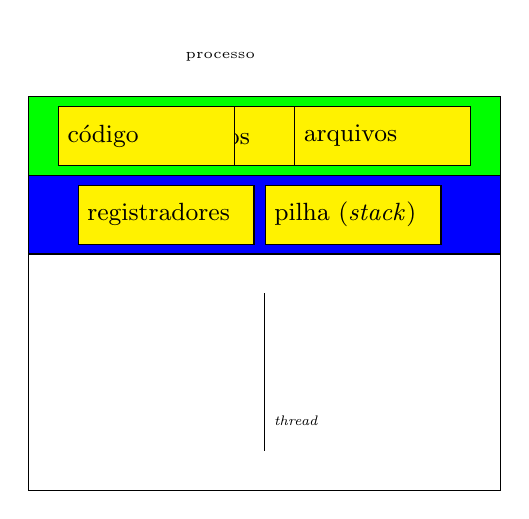
\begin{tikzpicture}[]
      \prochead{}
      \node[fill=blue,minimum width=6cm,minimum height=1cm,draw] (dynamic) [below of=text] {};
      \node[resources] (reg) [below of=code,xshift=0.5*\dx] {registradores};
      \node[resources] (stack) [right of=reg,xshift=2.75*\dx] {pilha (\emph{stack})};
      \node[minimum width=6cm,minimum height=5cm,draw] (threadsection) [below of=dynamic] {};
      \draw (0,-4*\dx) -- +(0,-2cm) node[anchor=south west] {\em thread};
    \end{tikzpicture}
  \end{center}
\end{block}

\end{frame}

\begin{frame}{\mysection}
  \begin{columns}
    \begin{column}{0.55\textwidth}
      \begin{block}{Múltiplas \emph{threads}}
        \bigskip
          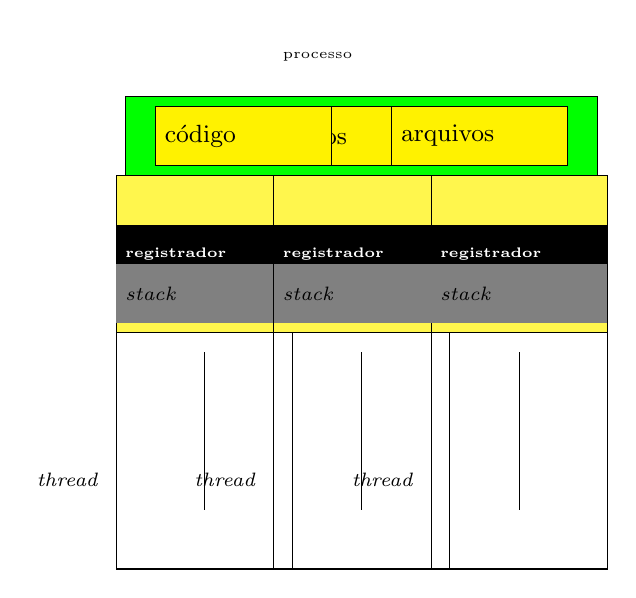
\begin{tikzpicture}
            \prochead{}
            \foreach \x in {-1,0,1} {
              \node[fill=yellow!70,minimum height=2cm,minimum width=2cm,draw] (dynamic\x) [below of=text,yshift=-.5cm,xshift=2*\x cm] {};
              \node[color=white,fill=black] (reg\x) at (dynamic\x)  {\bf\tiny registrador};
              \node[fill=gray] (stack\x) [below of=reg\x,yshift=.5cm] {\scriptsize\emph{stack}};
              \node[minimum height=3cm,minimum width=2cm,draw] (thread\x) [below of=stack\x,yshift=-1cm] {};
              \draw (2*\x cm,-5.5*\dx) -- +(0,-2cm) node[anchor=south east] {\scriptsize\emph{thread}};
            }
          \end{tikzpicture}
      \end{block}
    \end{column}
    \begin{column}{0.4\textwidth}
      \begin{block}{Benefícios}
        \begin{itemize}
        \item Responsividade;
        \item Compartilhamento de recursos;
        \item Economia;
        \item Utilização de arquiteturas multiprocessadas.
        \end{itemize}
      \end{block}
    \end{column}
  \end{columns}
  
\end{frame}


\def\mysection{Espaço de endereçamento do usuário}
\subsection{\mysection}
\tikzset{every node/.style={font=\scriptsize},
  userspace/.style={color=blue,fill=blue!40, minimum width=3cm,
    minimum height=7cm,text width=2.5cm,anchor=north},
  resource/.style={text width=2cm, minimum width=2.5cm,
    minimum height=1.5cm,fill=white}}
\colorlet{calcula}{green!50!black}
\colorlet{io}{blue!50!black}
\def\ashead{ % address space draw header
    \node[userspace] (useraddress) {};
    \node[] (label) [above of=useraddress,yshift=3cm] {espaço de endereçamento do usuário};
}

\begin{frame}{\mysection{} {\bf sem} {\em threads}}
  \begin{center}
  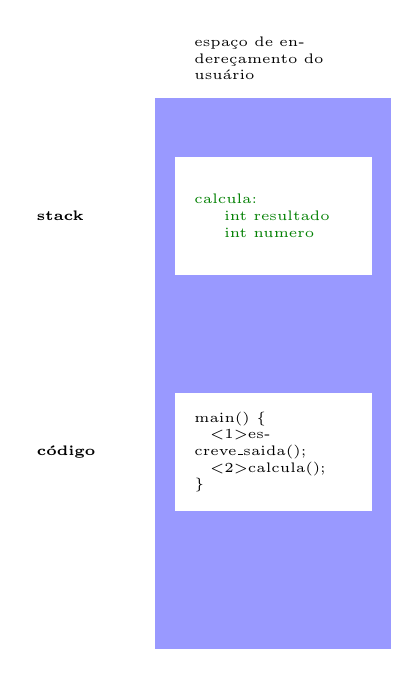
\begin{tikzpicture}
    \ashead
   \node<1>[color=blue,resource,align=left] (routine) [below of=label,yshift=-1cm] {escreve\_saida: \\ \tiny \hspace{.3cm} FILE $*$arquivo\\\hspace{.3cm} char $*$conteudo};
    \node<2>[calcula,resource,align=left] (routine) [below of=label,yshift=-1cm] {calcula: \\ \tiny \hspace{.3cm} int resultado\\\hspace{.3cm} int numero};
    \node [left of=routine,xshift=-1cm] {\bf stack};
    \node[resource,align=left] (code) [below of=routine,yshift=-2cm] 
    {main() $\{$\\\hspace{.2cm}{\tiny \alert<1>{escreve\_saida();} \\\hspace{.2cm}\alert<2>{calcula();}\\$\}$}};
    \node [left of=code,xshift=-1cm] {\bf código};
  \end{tikzpicture}
\end{center}
\end{frame}

\begin{frame}{\mysection{} {\bf com} {\em threads}}
\begin{center}
  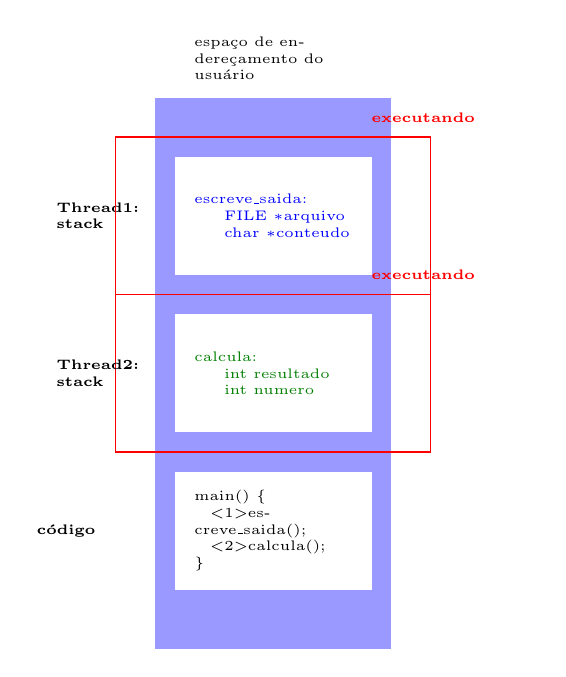
\begin{tikzpicture}[exec/.style={color=red,minimum width=4cm,minimum height=2cm,draw}]
    \ashead
   \node[color=blue,resource,align=left] (io) [below of=label,yshift=-1cm] {escreve\_saida: \\ \tiny \hspace{.3cm} FILE $*$arquivo\\\hspace{.3cm} char $*$conteudo};
   \node [left of=io,xshift=-1cm,text width=1.5cm] {\bf Thread1: stack};
   \node<1>[exec] (exec) at (io) {};
   \node<1>[color=red] [right of=exec,xshift=1.25cm,yshift=1.25cm] {\bf executando};
   \node[calcula,resource,align=left] (calcula) [below of=io,yshift=-1cm] {calcula: \\ \tiny \hspace{.3cm} int resultado\\\hspace{.3cm} int numero};
   \node<2>[exec] (exec) at (calcula) {};
   \node<2>[color=red] [right of=exec,xshift=1.25cm,yshift=1.25cm] {\bf executando};
    \node [left of=calcula,xshift=-1cm,text width=1.5cm] {\bf Thread2: stack};
    \node[resource,align=left] (code) [below of=calcula,yshift=-1cm] 
    {main() $\{$\\\hspace{.2cm}{\tiny \alert<1>{escreve\_saida();} \\\hspace{.2cm}\alert<2>{calcula();}\\$\}$}};
    \node [left of=code,xshift=-1cm] {\bf código};
  \end{tikzpicture}
\end{center}
\end{frame}

\def\mysection{Sequência de escalonamento}

\subsection{\mysection}

\tikzset{every node/.style={minimum height=.75cm,font=\tiny,text width=2cm},
  labelio1/.style={color=white,minimum width=1cm,fill=black},
  proc/.style={labelio1,minimum width=2cm},
  labelio2/.style={fill=red,minimum width=4cm},
  end/.style={fill=gray,minimum width=.25cm}
}
\begin{frame}{\mysection}
\scriptsize\def\nprocs{0}
\def\prelabelprocone{
  \ifnum\nprocs=0%
  {}
  \fi
  \ifnum\nprocs=1%
  {thread 1\\}
  \fi
  \ifnum\nprocs=2%
  {thread 1, CPU 1\\}
  \fi
}
\def\prelabelproctwo{
  \ifnum\nprocs=0%
  {}
  \fi
  \ifnum\nprocs=1%
  {thread 2\\}
  \fi
  \ifnum\nprocs=2%
  {thread 2, CPU 2\\}
  \fi
}
\def\schedhead{% header for scheduling
  \node<1-> (labelio) {\prelabelprocone \bf escreve\_saida()};
  \node<2-6,7-12,13-16,17>[labelio1,draw] (labelio1) [right of=labelio,xshift=1cm] {execução};
  \node<3-6,8-12,14-16,17>[labelio2,draw] (labelio2) [right of=labelio1,xshift=1.75cm] {bloqueio: requisição de E/S};
  \node<4-6,11-12,15-16,17>[labelio1,draw] (labelio3) [right of=labelio2,xshift=1.75cm] {execução};
  \node<5-6,12,16,17>[end] (endio) [right of=labelio3,xshift=1.25cm] {fim};
  \node<1-> (labelproc) [below of=labelio] {\prelabelproctwo \bf calcula()};
}

\begin{block}<1-6,17>{{\bf Sem} {\em threads}}
    \bigskip
    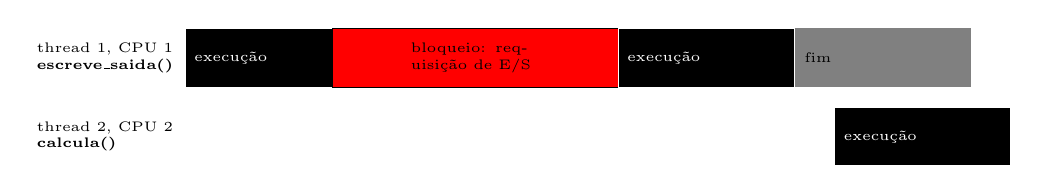
\begin{tikzpicture}
      \schedhead
      \node<6,17>[proc,draw] (proc) [right of=endio,yshift=-1cm,xshift=-.5cm] {execução};
    \end{tikzpicture}
  \end{block}

\begin{block}<7-12,17>{{\bf Com} {\em threads}, um processador}
    \bigskip\def\nprocs{1}
    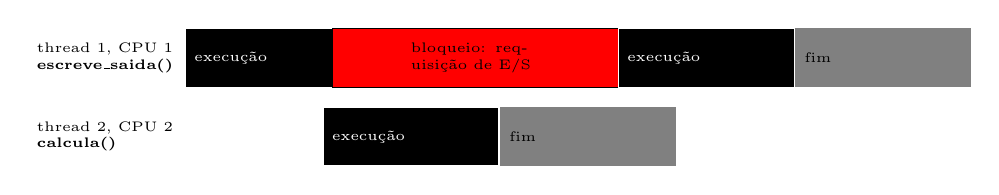
\begin{tikzpicture}
      \schedhead
      \node<9-12,17>[proc,draw] (proc) [right of=labelio1,yshift=-1cm,xshift=.75cm] {execução};
      \node<10-12,17>[end] (endproc) [right of=proc,xshift=1.25cm] {fim};
    \end{tikzpicture}
  \end{block}

\begin{block}<13-16,17>{{\bf Com} {\em threads}, vários processadores}
    \bigskip\def\nprocs{2}
    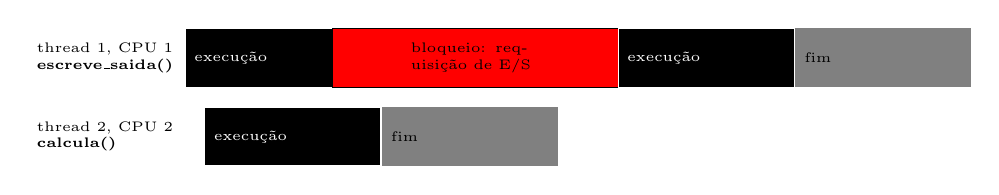
\begin{tikzpicture}
      \schedhead
      \node<13-16,17>[proc,draw] (proc) [right of=labelproc,xshift=1.25cm] {execução};
      \node<14-16,17>[end] (endproc) [right of=proc,xshift=1.25cm] {fim};
    \end{tikzpicture}
  \end{block}


\end{frame}

\begin{frame}{Exemplos de utilização de {\em threads}}

  \begin{itemize}
  \item \href{http://adrianoholanda.org/edu/os/proc/proc_thread_win32.c}{Win32}
  \item \href{http://adrianoholanda.org/edu/os/proc/proc_thread_posix.c}{PThreads}
  \end{itemize}
  
\end{frame}


\end{document}


\begin{frame}{Modelo muitos para um}{Modelos de múltiplas {\em threads}}
  \begin{columns}
    \begin{column}{0.4\textwidth}
      \begin{block}{múltiplas \em threads}
        \includegraphics[scale=0.6]{../img/proc_thread_Nx1.pdf}
      \end{block}
    \end{column}
    \begin{column}{0.6\textwidth}
      \begin{block}{Características}
        \begin{itemize}
        \item Gerenciamento no espaço do usuário;
        \item Chamada bloqueante de uma das {\em threads} bloqueia as outras;
        \item Somente um {\em thread} acessa o {\em kernel} por vez,
          fazendo com que as {\em threads} não possam ser executas em
          paralelo em ambiente multiprocessados. 
        \end{itemize}
      \end{block}
      \begin{block}{Quem implementa este modelo?}
        \begin{itemize}
        \item {\em Green threads} -- Solaris;
        \item \href{http://www.gnu.org/software/pth/}{GNU \em Portable Threads}.
        \end{itemize}
      \end{block}
    \end{column}
  \end{columns}
\end{frame}

\begin{frame}{Modelo um para um}{Modelo de múltiplas {\em threads}}
  \begin{columns}
    \begin{column}{0.375\textwidth}
      \begin{block}{múltiplas \em threads}
        \includegraphics[scale=0.6]{../img/proc_thread_1x1.pdf}
      \end{block}
    \end{column}
    \small
    \begin{column}{0.6\textwidth}
      \begin{block}{Características}
        \begin{itemize}
        \item Cada {\em thread} de usuário é associada a uma {\em
            thread} do {\em kernel};
        \item Chamada bloqueante de uma das {\em threads} \alert{não} bloqueia as outras;
        \item Várias {\em threads} podem ser executadas em paralelo em
          multiprocessadores;
        \item Custo adicional da criação de novas {\em threads} no
          espaço do {\em kernel} pode prejudicar o desempenho do sistema.
        \end{itemize}
      \end{block}
      \begin{block}{Quem implementa este modelo?}
        \begin{itemize}
        \item Linux;
        \item Windows 98/98/NT/2000/XP.
        \end{itemize}
      \end{block}
    \end{column}
  \end{columns}
\end{frame}

\begin{frame}{Modelo muitos para muitos}{Modelo de múltiplas {\em threads}}
  \begin{columns}
    \begin{column}{0.4\textwidth}
      \begin{block}{múltiplas \em threads}
        \includegraphics[scale=0.6]{../img/proc_thread_NxN.pdf}
      \end{block}
    \end{column}
    \begin{column}{0.6\textwidth}
      \begin{block}{Características}
        \begin{itemize}
        \item Multiplexa muitas {\em threads} do espaço do usuário
          para um número menor ou igual no espaço do {\em kernel};
        \item Não há limitação ao número de {\em threads} a ser criado
          no espaço do usuário, como acontece no modelo muitos para um;
        \item Em caso de uma chamada de sistema bloqueante realizada por 
           uma {\em thread}, o {\em kernel} pode escalonar outra {\em thread}.
        \end{itemize}
      \end{block}
      
    \end{column}
  \end{columns}
\end{frame}

\begin{frame}{Modelo de 2 níveis}{Modelo de múltiplas {\em threads}}
  \begin{columns}
    \begin{column}{0.45\textwidth}
      \begin{block}{múltiplas \em threads}
        \includegraphics[scale=0.6]{../img/proc_thread_2levels.pdf}
      \end{block}
    \end{column}
    \begin{column}{0.55\textwidth}
      \begin{block}{Características}
        \begin{itemize}
        \item Variação do modelo muitas para muitas que permite que no
          nível do usuário uma {\em thread} esteja ligada somente a
          uma {\em thread}.
        \end{itemize}
      \end{block}
        \begin{block}{Quem implementa este modelo?}
          \begin{itemize}
          \item {\sc IRIX};
          \item {\sc HP-UX};
          \item True64 {\sc UNIX}.
          \end{itemize}
        \end{block}
    \end{column}
  \end{columns}
\end{frame}
